\documentclass{article}
\usepackage[version=3]{mhchem}
\usepackage{graphicx}
\usepackage{csvsimple}
\usepackage{longtable}

\title{%
	MATH 376: Numerical Analysis \\
	\large  Project 3: Indoor Air Polution
	}
\author{Quan Vu}
\date{\today}

\begin{document}
	\maketitle
	
	\section{Abstract}
	This project deals with indoor air pollution in enclosed spaces such as homes, offices and work areas. We will be leveraging mathematical modelling to describe a real problems using abstract mathematical concepts. By solving for unknowns using these mathematical concepts, we relate the results back to the problem of air pollution and what we can do to improve air quality in these enclosed spaces.
	
	\section{Introduction}
	
	\subsection{Background information}
	In this project, we explore how to model certain real-life scenarios using systems of linear equations. The power of these linear systems will enable us to have valuable insights which we can use to make a positive impact on these scenarios.
	
	\subsection{Problem description}
	The problem is given using the figure depicted below. There is a restaurant whose serving area consists of two rooms for smokers and kids, together with one elongated room. Room 1 and 3 have sources of \ce{CO2} coming from smokers and a faulty grill. Rooms 1 and 2 also gain \ce{CO2} from air intakes that are positioned alongside the freeway.\\
	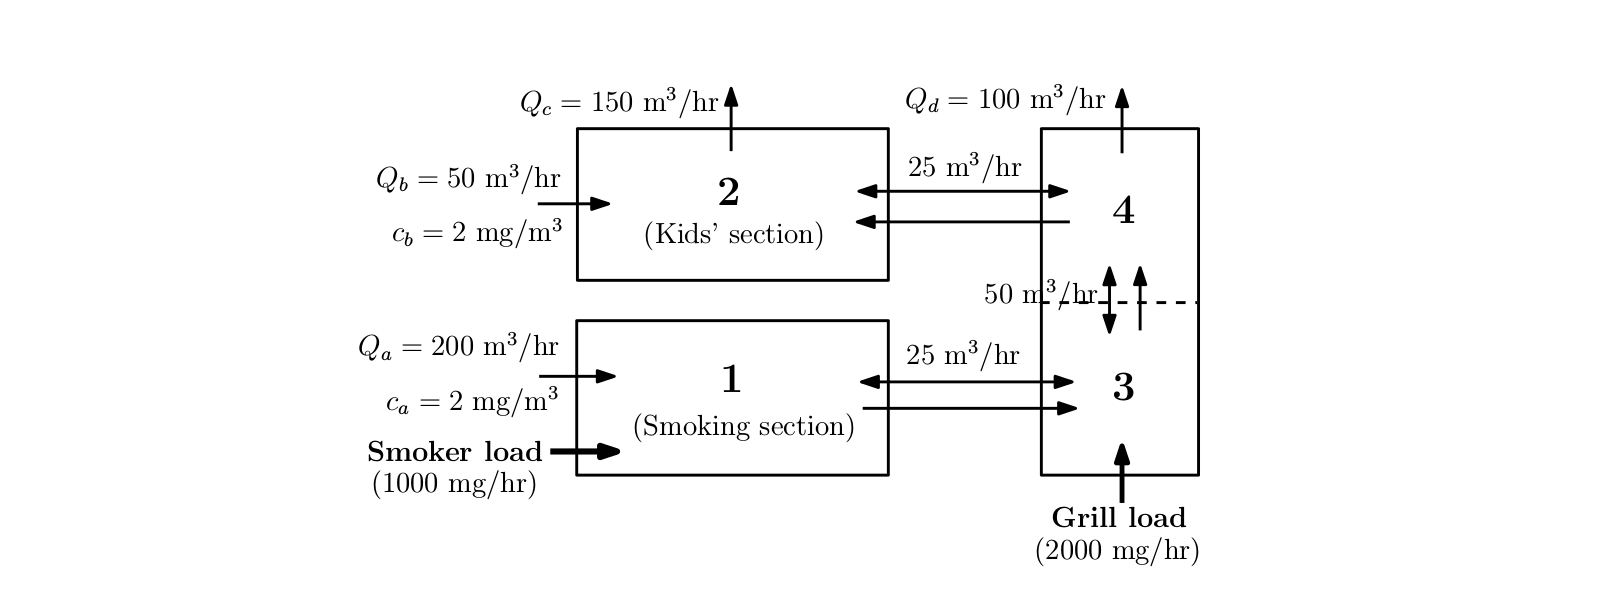
\includegraphics[scale=0.22]{Problem.png}
    
	\subsection{Outline}
	We can model the influx and outflux of \ce{CO2} in each room by using systems of linear equations. Since we know that the rooms are in steady states, the influx of \ce{CO2} must equal the outflux of \ce{CO2} for each of the rooms.
	
	\section{Numerical methods}
	In this section, we will use Gaussian elimination, LU factorization as well as the Jacobian method to solve systems of linear equations.\\
	
	Let ${c1, c2, c3, c4}$ be the concentrations of \ce{CO2} in rooms 1, 2, 3 and 4, respectively. Then from the diagram, we construct the steady-state equations, assuming that outflux must equal influx in the long run:
	
	\[225{\times}c1 + 25{\times}c3 = -1400\]
	\[175{\times}c2 - 125{\times}c4 = 100\]
	\[225{\times}c1 - 275{\times}c3 + 50{\times}c4 = -2000\]
	\[25{\times}c2 + 250{\times}c3 - 275{\times}c4 = 0\]
	
	\section{Results}
    
    \subsection{Using Gaussian elimination}
    Gaussian elimination results in the following:
    ${c1 = 8.0996 mg/m^3}$, ${c2 = 12.3448 mg/m^3}$, ${c3 = 16.8966 mg/m^3}$, and ${c4 = 16.4828 mg/m^3}$
    \subsection{Using LU Factorization}
    The built-in LU factorization method in Matlab results in the exact same results:
    ${c1 = 8.0996 mg/m^3}$, ${c2 = 12.3448 mg/m^3}$, ${c3 = 16.8966 mg/m^3}$, and ${c4 = 16.4828 mg/m^3}$
    \subsection{Using Jacobi method}
    The Jacobi method requires that the matrix must be strictly diagonally dominant in order for the method to converge. Luckily, our matrix satisfies this requirement. Using the intial guesses where all concentrations are ${1 mg/m^3}$, the method converges after 24 iterations, with tolerance ${10^{-6}}$. The results are  ${c1 = 8.0996 mg/m^3}$, ${c2 = 12.3448 mg/m^3}$, ${c3 = 16.8965 mg/m^3}$, and ${c4 = 16.4827 mg/m^3}$
    \subsection{Discussion}
    \subsubsection{Question c}
    Quite surprisingly, room 1, the designated smoker's room, actually has the lowest concentration of \ce{CO2}. However upon closer inspection, we see that room 1 is very well ventilated, with the outflux measured in ${225 \times c1}$. Room 3 has the highest concentration of \ce{CO2}, because it receives the large outflux of room 1 as parts of its influx. Even though room 3 is quite well ventilated (outflux is measured at ${275 \times c3}$, the heavy influx coming from the grill and from room 1 hold the concentration of \ce{CO2} in this room at a high level.
    \subsubsection{Question d}
    The inverse of the coefficient matrix A is given by Matlab's inv function:
     \[
   		A^{-1}=
  		\left[ {\begin{array}{cccc}
   		0.004996168582375 &  0.000015325670498 & -0.000551724137931 & -0.000107279693487\\
   		0.003448275862069 & 0.006206896551724 & -0.003448275862069 & -0.003448275862069\\
   		0.004965517241379 & 0.000137931034483 & -0.004965517241379 & -0.000965517241379\\
   		0.004827586206897 & 0.000689655172414  & -0.004827586206897 & -0.004827586206897\\
  		\end{array} } \right]
	\]
	Let the constant matrix be \emph{b}, where:
	\[
   		b=
  		\left[ {\begin{array}{c}
   		1400\\
   		100\\
   		-2000\\
   		0\\
  		\end{array} } \right]
	\]
	then we know that the concentration of \ce{CO2} in the second room is precisely the the dot product of the second row of ${A^{-1}}$ and ${b^{T}}$.\\
	As such, the smokers contribute around
	\[\frac{1000}{1400} \times \frac{1400 \times 0.003448275862069}{12.3448} \times 100\% \approx 27.9\%\]
	As for the grills:
	\[\frac{-2000 \times -0.003448275862069}{12.3448} \times 100\% \approx 55.9\%\]
	The rest, ${16.2\%}$, comes from the intake vents.
    \subsubsection{Question e}
    Suppose now smoking is banned, and the grill is fixed. We see that \ce{CO2} contribution in the constant matrix would drop to 400 for the first entry, and 0 for the third. Using Matlab to solve with a new constant matrix, we obtain that the concentration is ${2 mg/m^3}$ for every room.
    \subsubsection{Question f}
    Now suppose that the mixing between areas 2 and 4 is decreased to ${5m^3/hr}$. Then we have a new system:
    \[225{\times}c1 + 25{\times}c3 = -1400\]
	\[155{\times}c2 - 105{\times}c4 = 100\]
	\[225{\times}c1 - 275{\times}c3 + 50{\times}c4 = -2000\]
	\[5{\times}c2 + 250{\times}c3 - 255{\times}c4 = 0\]
	
	The concentration in room 2 drops to 12.0800, which makes sense since room 2 is getting its \ce{CO2} intake from the air circulating in the other 3 rooms. Decreasing the amount of air flowing between 2 and 4 would help reduce the concentration in room 2. However the drop is not too significant since from room 4, there is still a significant portion of volumetric airflow flowing into room 2 at ${100m^3/h}$.
	
\end{document}